\documentclass[12pt]{extarticle}
\oddsidemargin=0.0in
\evensidemargin=0.0in
\textwidth=6.5in
\topmargin=-0.75in
\textheight=9.5in
%\usepackage{hyperref}
\usepackage{url}
\usepackage{graphicx}
\usepackage{amsmath}

\begin{document}
\pagestyle{empty}
 
\begin{center}
{\LARGE {\bf Homework Ten}}\\
\bigskip
{\Large {\bf Calculus I}}\\
\bigskip
{\Large {\bf College of the Atlantic}}\\
\bigskip
{ {\bf Due Friday, November 18, 2022}}\\ 
\end{center}
\medskip

%\noindent There are two parts to this assignment.\\

\noindent {\bf Part 1: WeBWorK}.  Do Homework 10 on
WeBWorK.  The WeBWorK page is here: 
\url{https://webwork.runestone.academy/webwork2/coa-feldman-es1024i-fall-2022/}.
I recommend doing the WeBWorK part of the homework first.  This will
enable you to benefit WeBWorK's instant feedback before you do part
two.\\ 


\noindent {\bf Part 2: Non-WeBWorK problems}.  Here are some
instructions for how to submit this part of the assignment.
\begin{itemize}
  \setlength{\itemsep}{0mm}
\item Do the problems by hand using pencil (or pen) and paper.
  There is no need to type this assignment.
%\item If you like working on a tablet, go for it. 
\item Make a pdf scan of your work using genius scan or some
  similar scanning app.  Please make the homework into a single
  pdf, not multiple pdfs.
\item Submit the assignment on google classroom.  Please don't
  email it to me.
  %(Between my two classes I will be receiving
  %around 60 assignments a week.  Keeping track of them all in email 
  %is challenging.)
%\item If you want, you can do the non-WeBWorK problems in pairs and
%  submit only one assignment for the two of you. 
\end{itemize}

\noindent Here are some non-WeBWorK problems.


\begin{enumerate}
\setlength{\itemsep}{3mm}

\item You have a piece of cardboard that is 4 inches by two
  inches. You wish to use the cardboard to make a rectangular box. To
  do so you will cut an $x$ by $x$ square out of each corner and the
  fold up along the dotted lines, as shown in the figure. What value
  of $x$ leads to the box with the greatest volume?

\begin{figure}[h!]
\begin{center}
\vspace{1mm}
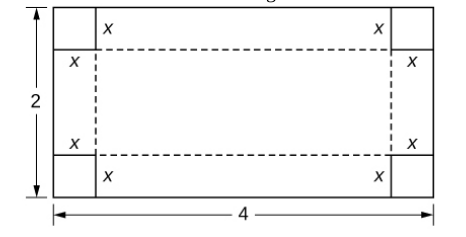
\includegraphics[width=3.7in]{box.png}
\vspace{-2mm}
%\caption{The amount of energy used by a flying bird.}
\label{fig:towns}
\vspace{-1mm}
\end{center}
\end{figure}

\item {\bf Optional Challenge Problem.} A spherical rock on a beach on
  the coast of Maine erodes at a rate proportional to its surface
  area. As it erodes it maintains its spherical shape. The rock erodes
  in such a way that it loses half of its volume in 40 years.  How
  long will it take for the rock to erode completely?
\end{enumerate}

\end{document}




  \item Determine an equation for the linear function that generates
    the values in the table below.  

\begin{center}
\begin{tabular}{|| l | l ||}
\hline $x$ & $f(x)$ \\
\hline
5.2 & 27.8 \\
5.3 & 29.2 \\
5.4 & 30.6 \\
5.5 & 32.0 \\
5.6 & 33.4 \\
\hline
\end{tabular}
\end{center}





\end{document}
